\section{Der Algorithmus}\label{kap_algorithmus}
Im Folgenden wird zunächst der Algorithmus aus dem Paper \cite{cima_paper} beschrieben und erklärt, sowie im Anschluss einige Modifikationen erläutert, mit denen in dieser Bachelorarbeit weitergearbeitet werden soll.\\
Der Algorithmus berechnet für einen gegebenen Baum mit Kantengewichten $\omega \geq 1$ die Mindestanzahl an Agenten, die den Baum dekontaminieren können. Außerdem gibt er an, welcher Knoten der Startpunkt dieser Agenten ist.


\subsection{Ursprünglicher Algorithmus (Grundlage)}\label{paperAlgoChapter}

Zu Beginn des Algorithmus aus \cite{cima_paper}, werden die Knotengewichte aller Knoten berechnet. Dieses ergibt sich jeweils aus dem maximalen Kantengewicht aller inzidenter Kanten. 

\begin{mydef}
	Sei $\omega(e) \in \mathbb N_{> 0}$ das Kantengewicht der Kante $e$. Dann gilt für das Knotengewicht $\omega(x)$ des Knoten x:   $$\omega(x) = \max_{e} \omega(e)$$ für jede zu $x$ inzidente Kante $e$.
\end{mydef}

Das Knotengewicht gibt an, wie viele Agenten als Wachen benötigt werden, um den aktuellen Knoten x, bzw. den dazugehörigen Teilbaum, vor einem kontaminierten Teilbaum zu schützen.
\\
\\
Nachdem für alle Knoten die entsprechenden Gewichte berechnet wurden, werden zwischen den Baumknoten Nachrichten verschickt. Diese Nachrichten beinhalten die Information, wie viele Agenten benötigt werden, um den entsprechenden Teilbaum zu dekontaminieren.  

\begin{mydef}\label{def_nachricht}
	Eine Nachricht $\lambda_{y}(e)$ wird von einem Knoten $x$ zu einem Knoten $y$ über die Kante $e$ im Baum verschickt. Diese erhält Informationen über den Teilbaum von $x$, die von Knoten $y$ zur Berechnung der Agenten benötigt werden.
\end{mydef}

Die Nachrichten werden nach folgender Rekursionsformel \cite{cima_paper} berechnet:\\
Sei $e = \{x, y\}$ eine Kante inzident zu $y$ und $\lambda_{y}(e)$ die Nachricht, die über $e$ nach $y$ geschickt wird. Ist $x$ ein Blatt des Baumes, so gilt $\lambda_{y}(e) = \omega(x)$. Ansonsten seien $z_{1}, ..., z_{deg(x)-1}$ die Nachbarn von $x$ ohne $y$, wobei $deg(x)$ der Knotengrad von $x$ ist.  Außerdem gilt $l_{i} = \lambda_{x}(\{x, z_{i}\})$ und sei o.B.d.A. $l_{i} \geq l_{i+1}$ \cite{cima_paper}: $$\lambda_{y}(e) = max \{l_{1}, l_{2} + \omega(x)\}$$

\subsubsection{Berechnung der Nachrichten}

Um ein besseres Verständnis für die Rekursionsgleichung zu erhalten, und es für die Implementierung anschaulicher ist, den Algorithmus durch eine Fallunterscheidung zu betrachten, werden im Folgenden drei Fälle erläutert, die im Algorithmus auftauchen können:\\\\	
Es gibt drei verschiedene Fälle, wie Nachrichten berechnet und verschickt werden können:

\begin{enumerate}
	
	\item Fall:
		
%		\begin{minipage}{1\textwidth} 
		
		
%		\begin{wrapfigure}{r}{0.65\textwidth}
%			\begin{center}
%				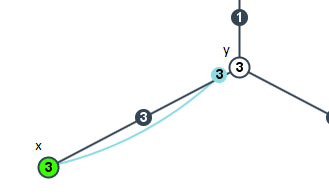
\includegraphics[width=1\textwidth]{bilder/abb_blattknoten.png}
%			\end{center}
%			\caption{Das Knotengewicht des Blattknotens x (grün) bestimmt den Wert Nachricht $\lambda_{y} = 3$ (blau) zum Nachbarknoten y.}
%			\label{abb_leaf}
%		\end{wrapfigure}
			
		Zu Beginn des Algorithmus, oder falls keine weitere Nachricht mehr berechnet werden kann, sendet ein beliebiger Blattknoten, der noch keine Nachricht versendet hat, seine Nachricht an den eigenen Nachbarn.\\
		
		Die zu sendende Nachricht $\lambda_{y}$ vom Blatt $x$ an seinen Nachbarknoten $y$ ist dabei nur das eigene Gewicht (Abbildung \ref{abb_leaf}): Es gilt daher $$\lambda_{y} = \omega(x)$$
		%		\end{minipage}
		%		\hfill
		%		\begin{minipage}{0.35\textwidth}
		
%		\begin{figure}[htb]
%			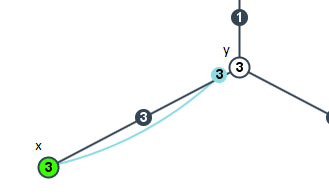
\includegraphics[width=0.65\textwidth]{bilder/abb_blattknoten.png}
%			\captionsetup{width=0.65\textwidth}
%			\caption{Das Knotengewicht des Blattknotens $x$ (grün) bestimmt den Wert Nachricht $\lambda_{y} = 3$ (blau) zum Nachbarknoten $y$.}
%			\label{abb_leaf}
%		\end{figure}

%		\end{minipage}
		
	
			
	\item Fall:\label{algo_fall_2}
	
		
		Der aktuelle Knoten $x$ hat genau $n-1$ Nachrichten erhalten, wobei $n$ die Anzahl der inzidenten Knoten ist. Also hat er von jedem Nachbarn, außer von dem Knoten $y$, eine Nachricht erhalten.
		
%		\begin{minipage}{1\textwidth} 
	
%		\begin{wrapfigure}{r}{0.65\textwidth}
%			\begin{center}
%				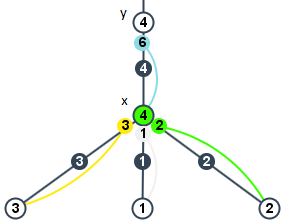
\includegraphics[width=1\textwidth]{bilder/abb_paper_n-1knoten.png}
%			\end{center}
%			\caption{Der Wert der neuen Nachricht $\lambda_{y}$(blau) von Knoten x zu Knoten y beträgt 6, da $l_{2} + \omega(x) = 6$ (grün) größer ist als $l_{1} = 3$ (gelb).}
%			\label{abb_n-1}
%		\end{wrapfigure}
		
		Um eine Nachricht von $x$ an den Nachbarknoten $y$ zu senden, der bis zu diesem Zeitpunkt noch keine Nachricht an $x$ gesendet hat, nimmt man die zwei größten Nachrichten ($l_{1}$ und $l_{2}$), die bei $x$ angekommen sind. Mit diesen beiden angekommenen Nachrichten $l_{1} \ge l_{2}$ sowie dem Knotengewicht $\omega(x)$ wird die Nachricht $\lambda_{y}$ an $y$ wie folgt berechnet (siehe auch Abbildung \ref{abb_n-1}): $$\lambda_{y} = max\{l_{1},  l_{2} + \omega(x)\}$$
		Nach dem Berechnen und Versenden der Nachricht $\lambda_{y}$ muss $x$ auf die letzte ankommende Nachricht (von $y$) warten. Sobald diese Nachricht angekommen ist, berechnet $x$ die Nachrichten für alle anderen Nachbarknoten, wie im Fall \ref{labelAufUnterfall} beschrieben. 
	%				\end{minipage}
	%				\hfill
	%				\begin{minipage}{0.35\textwidth}
		
		
%		\begin{figure}[htb]
%			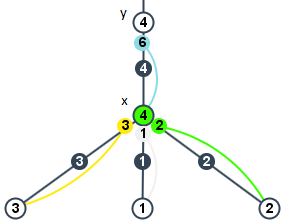
\includegraphics[width=0.65\textwidth]{bilder/abb_paper_n-1knoten.png}
%			\captionsetup{width=0.65\textwidth}
%			\caption{Der Wert der neuen Nachricht $\lambda_{y}$(blau) von Knoten $x$ zu Knoten $y$ beträgt 6, da $l_{2} + \omega(x) = 6$ (grün) größer ist als $l_{1} = 3$ (gelb).}
%			\label{abb_n-1}
%		\end{figure}
		
%		\end{minipage}
		
		
	\item Fall:
	
		Der aktuelle Knoten $x$ hat bereits von allen $n$ zu ihm inzidenten Knoten eine Nachricht erhalten, selbst jedoch noch nicht zu allen Knoten eine Nachricht gesendet. Diese Nachrichten müssen nun berechnet und versendet werden.\label{labelAufUnterfall}
		
		
%		\begin{minipage}{1\textwidth} 
			
			
%		\begin{wrapfigure}{r}{0.65\textwidth}
%			\begin{center}
%				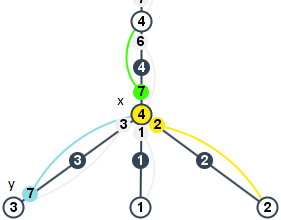
\includegraphics[width=1\textwidth]{bilder/abb_paper_nknoten.png}
%			\end{center}
%			\caption{Die neue Nachricht $\lambda_{y}$ (blau) von Knoten x zu Knoten y hat den Wert 7, da $l_{1} = 7$ (grün) größer ist als $l_{2} + \omega(x) = 6$ (gelb).}
%			\label{abb_n}
%		\end{wrapfigure}
		
		Um eine Nachricht von $x$ an einen Nachbarknoten $y$ zu senden, der bis zu diesem Zeitpunkt noch keine Nachricht von $x$ erhalten hat, wird ähnlich wie in Fall \ref{algo_fall_2} vorgegangen: Man nimmt die zwei größten Nachrichten ($l_{1}$ und $l_{2}$), die bereits bei $x$ angekommen sind, aber nicht von Knoten $y$ stammen. Bei der Bestimmung von $l_{1}$ und $l_{2}$ von $y$ wird also die Nachricht $\lambda_{x}$, welche von $y$ kam, ignoriert. Mit den beiden ermittelten Nachrichten $l_{1} \ge l_{2}$ sowie dem Knotengewicht $\omega(x)$ wird die Nachricht $\lambda_{y}$ an y wie folgt berechnet (Abbildung \ref{abb_n}):  $$\lambda_{y} = max\{l_{1},  l_{2} + \omega(x)\}$$
		Diese Berechnung wird für jeden Nachbarknoten von $x$ wiederholt, so dass jeder Nachbar eine Nachricht von $x$ erhält. Nach diesem Schritt ist die Bearbeitung des Knoten $x$ abgeschlossen, da er sowohl von jedem Nachbarn eine Nachricht erhalten hat, als auch an jeden Nachbarn eine Nachricht gesendet hat.
%				\end{minipage}
%				\hfill
%				\begin{minipage}{0.35\textwidth}
		
		
%		\begin{figure}[htb]
%			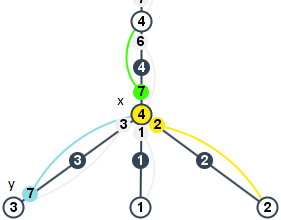
\includegraphics[width=0.65\textwidth]{bilder/abb_paper_nknoten.png}
%			\captionsetup{width=0.65\textwidth}
%			\caption{Die neue Nachricht $\lambda_{y}$ (blau) von Knoten $x$ zu Knoten y hat den Wert 7, da $l_{1} = 7$ (grün) größer ist als $l_{2} + \omega(x) = 6$ (gelb). Die Nachricht von $y$ zu $x$ (mit dem Wert = 3) wird bei dieser Berechnung ignoriert.}
%			\label{abb_n}
%		\end{figure}
		
%		\end{minipage}
	
		
		
\end{enumerate}

\begin{figure}[htbp]
	\subfigure[Das Knotengewicht des Blattknotens $x$ (grün) bestimmt den Wert Nachricht $\lambda_{y} = 3$ (blau) zum Nachbarknoten $y$.
	\label{abb_leaf}]{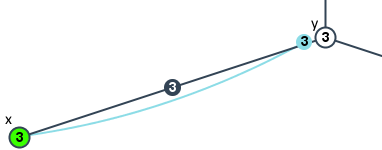
\includegraphics[width=0.7\textwidth]{bilder/abb_blattknoten_NEU2.png}}
	%	\hfill  
	%lösche die neue line und füge das \hfill wieder ein um die bilder nebeneiander zu haben
		
	\subfigure[Der Wert der neuen Nachricht $\lambda_{y}$(blau) von Knoten $x$ zu Knoten $y$ beträgt 6, da $l_{2} + \omega(x) = 6$ (grün) größer ist als $l_{1} = 3$ (gelb). \label{abb_n-1}]{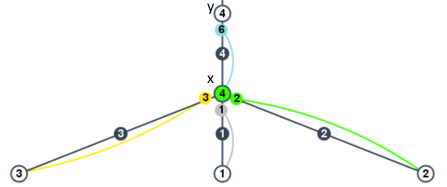
\includegraphics[width=0.7\textwidth]{bilder/abb_paper_n-1knoten_NEU2.png}} 
	%	\hfill
	
	\subfigure[Die neue Nachricht $\lambda_{y}$ (blau) von Knoten $x$ zu Knoten y hat den Wert 7, da $l_{1} = 7$ (grün) größer ist als $l_{2} + \omega(x) = 6$ (gelb). Die Nachricht von $y$ zu $x$ (mit dem Wert = 3) wird bei dieser Berechnung ignoriert. \label{abb_n}]{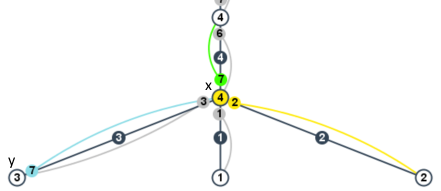
\includegraphics[width=0.7\textwidth]{bilder/abb_paper_nknoten_NEU2.png}}  
	
	\caption{Drei Fälle, die bei dem Algorithmus auftreten können. (Quelle: Eigene Darstellung im Applet)} 
	
\end{figure}


%\subsubsection{Berechnung der minimalen Agenten}

\subsubsection{Berechnung der minimalen Agentenzahl}

\begin{mydef}
	$\mu(x)$ bezeichnet man als Agentenzahl, welche benötigt wird, um den gesamten Baum vom Knoten x aus zu dekontaminieren. 
\end{mydef}

\begin{mydef}\label{def_homebase}
	Die Homebase ist ein beliebiger Knoten x im Baum, für den gilt: $\mu(x) = \min \mu(i)$ für alle Knoten i im Baum.
\end{mydef}

Sobald alle Knoten sowohl an alle Nachbarn eine Nachricht geschickt haben, als auch von allen Nachbarn eine Nachricht erhalten haben (jede Kante im gesamten Baum überträgt genau zwei Nachrichten), hat jeder Knoten $x$ alle Informationen, die gebraucht werden, um die minimale Anzahl an Agenten $\mu(x)$ zu errechnen, die benötigt werden, um den gesamten Baum von diesem Knoten aus zu dekontaminieren.
\\
\\
Die minimale Agentenanzahl $\mu(x)$, die am Knoten $x$ benötigt wird, wird wie folgt berechnet:
$$\mu(x) = max\{l_{1},  l_{2} + \omega(x)\},$$ wobei analog zu der Berechnung der Nachrichten gilt: $l_{1} \ge l_{2}$ sind die größten beiden angekommenen Nachrichten und $\omega(x)$ ist das Knotengewicht von $x$.
\\
\\
Nachdem alle Knoten $i$ ihr $\mu(i)$ berechnet haben, wird ein Knoten mit minimalem $\mu$ ausgewählt. Dieser ist die neue Homebase, von dem aus $\mu$ viele Agenten den gesamten Baum dekontaminieren können, ohne die Monotonie-Eigenschaft zu verletzen (siehe Definition \ref{def_monotonie}).


\subsubsection{Laufzeit}

	\begin{theorem}\label{thm_laufzeit}
		Der Algorithmus hat eine lineare Laufzeit.
	\end{theorem}
	\begin{proof}
		Die Anzahl der Nachrichten, die während des Algorithmus berechnet werden, ist linear in der Knotenzahl. Jeder Knoten sendet an jeden Nachbarn genau eine Nachricht und erhält auch von jedem Nachbarknoten genau eine Nachricht. Über jede Kante des Baumes werden daher zwei Nachrichten verschickt. Da die Anzahl an Kanten in einem Baum linear ist, werden auch nur linear viele Nachrichten berechnet und verschickt.\\\\
		Die Berechnung der Nachrichten erfolgt in konstanter Zeit, da nach einer Fallunterscheidung nur eine einfache Berechnung durchgeführt werden muss ($\lambda_{y} = max\{l_{1},  l_{2} + \omega(x)\}$).\\\\
		Nachdem alle Nachrichten verschickt wurden, muss jeder Knoten in konstanter Zeit das entsprechende $\mu$ berechnen.\\
		Im Anschluss kann durch einen erneuten Durchlauf durch alle Knoten das kleinste $\mu$ bestimmt werden, um die Homebase festzulegen.
		\\
		\\
		Einen etwas formaleren Beweis lässt sich in \cite{cima_paper} finden.
	\end{proof}

\newpage

\subsection{Modifikationen am Algorithmus}\label{modifizierterAlgoChapter}


%	\begin{wrapfigure}{l}{0.65\textwidth}
%		\begin{center}
%			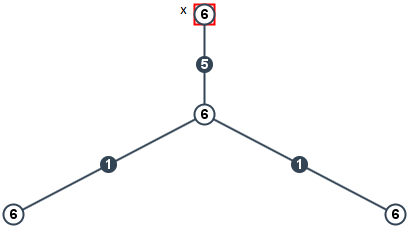
\includegraphics[width=1\textwidth]{bilder/abb_paper_problem.png}
%		\end{center}
%		\caption{Problem mit dem Algorithmus aus dem Paper. Der Knoten x sollte intuitiv mit 5 Agenten auskommen}
%		\label{fig:negBeispielPaperAlgo}
%	\end{wrapfigure}

Die Ergebnisse des im Artikel beschriebenen Algorithmus stimmen in einigen Fällen nicht mit der Intuition überein, die man bekommt, wenn man einige Beispielbäume betrachtet. Hierzu schauen wir uns Abbildung \ref{fig:negBeispielPaperAlgo} an. In dem  angegebenen Beispiel steht in jedem Knoten das entsprechende $\mu$, also die Anzahl an Agenten, die benötigt werden, um von dort aus den gesamten Baum zu dekontaminieren. Der Knoten $x$ sollte mit fünf Agenten auskommen: Alle fünf Agenten gehen über die erste Kante zum mittleren Knoten. Von dort aus werden nur noch zwei Agenten benötigt: Einer hält Wache, um die Monotonie zu gewährleisten, und der zweite dekontaminiert ein Blatt. Zum Schluss wird das letzte Blatt von einem Agenten dekontaminiert und der Algorithmus ist fertig.

		\begin{figure}[htb]
			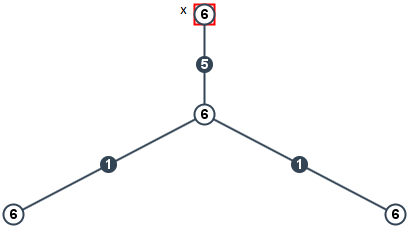
\includegraphics[width=0.65\textwidth]{bilder/abb_paper_problem.png}
			\captionsetup{width=0.65\textwidth}
			\caption{Beispiel, warum die modifizierte Variante des Algorithmus benutzt wird. Der Knoten $x$ sollte intuitiv mit 5 Agenten auskommen. (Quelle: Eigene Darstellung im Applet)}
			\label{fig:negBeispielPaperAlgo}
		\end{figure}

Der Unterschied zwischen dem originalen Algorithmus aus \cite{cima_paper} und der Intuition ist Folgender: Der ursprüngliche Algorithmus plant im Beispiel für den mittleren Knoten fünf Wachen ein (das Knotengewicht ist 5), obwohl die Agenten über die Kante mit Gewicht 5 gekommen sind, und diese dadurch dekontaminiert ist. Es ist daher nicht nötig, diese Kante zu bewachen, und es werden mehr Agenten eingeplant, als wirklich benötigt werden.
\\
Da das Problem, wie erläutert, am Knotengewicht liegt, wird im Folgenden eine Variante des Algorithmus beschrieben, die anders mit dem Knotengewicht umgeht. Allerdings kommt es zu Fehlern, wenn man nur das Knotengewicht verändert, weshalb zusätzliche Fälle in den Algorithmus eingebaut werden müssen, damit dieser sowohl richtig funktioniert, als auch das gerade beschriebene Problem löst.
\\
\\
Im Gegensatz zum originalen Algorithmus \cite{cima_paper} wird im modifizierten Algorithmus nicht mehr das Knotengewicht in die direkte Berechnung der Nachricht mit einbezogen, sondern dient nur noch zur Überprüfung, ob die berechnete Nachricht nicht zu klein ist. Außerdem wird mit den inzidenten Kanten und den bereits angekommenen Nachrichten - wie nachfolgend beschrieben - etwas anders umgegangen.

\subsubsection{Modifizierte Berechnung der Nachrichten}

Die Berechnung der Nachrichten aus dem Algorithmus in Kapitel \ref{paperAlgoChapter} muss wie folgt abgeändert werden:

\begin{enumerate}[label=\alph*)]
	
	\item 
		Um eine Nachricht von $x$ an einen Nachbarknoten $y$ zu senden, der bis zu diesem Zeitpunkt noch keine Nachricht von $x$ erhalten hat, nimmt man die Kantengewichte der zwei größten Kanten ($edge_{1}$ und $edge_{2}$), die inzident zu $x$ sind, jedoch nicht zu $y$. Mit den beiden ermittelten Kantengewichten, für die gilt $edge_{1} \ge edge_{2}$, wird die Nachricht $\lambda_{y}$ an $y$, wie auch in Abbildung \ref{modifiziert_a} gezeigt, berechnet:
		$$\lambda_{y} = edge_{1} + edge_{2}$$
		Vor der Bestimmung der zwei maximalen Kanten werden $edge_{1}$ und $edge_{2}$ auf 0 initialisiert, so dass die Berechnung auch funktioniert, falls es weniger als zwei Kanten gibt, auf die die Bedingung inzident zu $x$ und nicht inzident zu $y$ zutrifft (zum Beispiel bei einem Blattknoten).
	
	\item
		Nachdem die neue Nachricht $\lambda_{y}$ nun berechnet wurde, muss noch überprüft werden, ob $\lambda_{y}$ nicht kleiner ist als das Knotengewicht $\omega(x)$. Ist dies der Fall, bedeutet das, dass das Kantengewicht der Kante, über welche die Nachricht nach $y$ geschickt werden soll, größer ist als die berechnete Nachricht. Da dies nicht sein darf, weil sonst nicht genug Agenten zur Verfügung stehen, um über die Kante zu laufen, muss die Nachricht, die an $y$ geschickt werden soll, entsprechend angepasst werden (Beispiel in Abbildung \ref{modifiziert_b}):
		
		\begin{algorithmic}
			\If {$\lambda_{y} \leq \omega(x)$}
			\State $\lambda_{y} \gets \omega(x)$
			\EndIf
		\end{algorithmic}
	
	\item
		Außerdem darf die berechnete Nachricht $\lambda_{y}$ nicht kleiner sein als die größte in $x$ angekommene Nachricht $l_{1}$ (außer der Nachricht, die evtl. schon von $y$ erhalten worden ist). Ist die Nachricht $\lambda_{y}$ kleiner als $l_{1}$, würden nicht genug Agenten zur Verfügung stehen, um den Teilbaum, aus dem $l_{1}$ kommt, zu dekontaminieren. $\lambda_{y}$ muss kontrolliert und evtl. wie in Abbildung \ref{modifiziert_c} angepasst werden:
		
		\begin{algorithmic}
			\If {$\lambda_{y} \leq l_{1}$}
			\State $\lambda_{y} \gets l_{1}$
			\EndIf
		\end{algorithmic}
	
\end{enumerate}

Alle weiteren Erweiterungen des Algorithmus, die in dieser Bachelorarbeit erklärt und benutzt werden, beziehen sich auf diese Modifikation des Grundalgorithmus.

%\begin{figure}
%	\floatbox[{\capbeside\thisfloatsetup{capbesideposition={right,top},capbesidewidth=4cm}}]{figure}[\FBwidth]
%	{\caption{A test figure with its caption side by side}\label{fig:test}}
%	{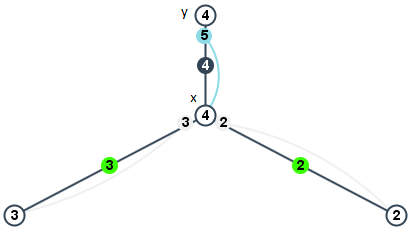
\includegraphics[width=0.75\textwidth]{bilder/abb_neu_max1max2.png}}
%\end{figure}
%
%\begin{figure}
%	\centering
%	\begin{subfigure}[b]{0.3\textwidth}
%		\floatbox[{\capbeside\thisfloatsetup{capbesideposition={right,top},capbesidewidth=4cm}}]{figure}[\FBwidth]
%		{\caption{A test figure with its caption side by side}\label{fig:test}}
%		{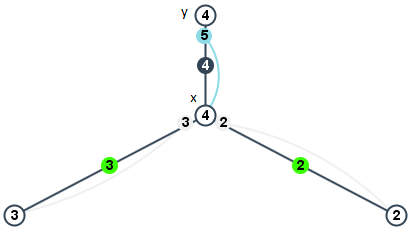
\includegraphics[width=0.75\textwidth]{bilder/abb_neu_max1max2.png}}
%	\end{subfigure}
%	
%	\begin{subfigure}[b]{0.3\textwidth}
%		\floatbox[{\capbeside\thisfloatsetup{capbesideposition={right,top},capbesidewidth=4cm}}]{figure}[\FBwidth]
%		{\caption{A test figure with its caption side by side}\label{fig:test}}
%		{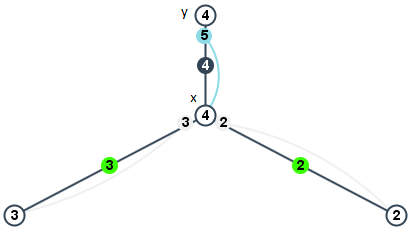
\includegraphics[width=0.75\textwidth]{bilder/abb_neu_max1max2.png}}
%	\end{subfigure}
%	
%	\begin{subfigure}[b]{0.3\textwidth}
%		\floatbox[{\capbeside\thisfloatsetup{capbesideposition={right,top},capbesidewidth=4cm}}]{figure}[\FBwidth]
%		{\caption{A test figure with its caption side by side}\label{fig:test}}
%		{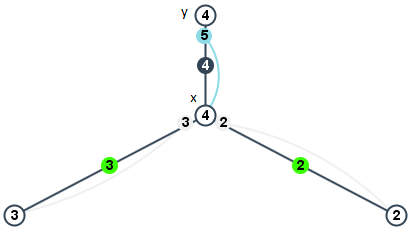
\includegraphics[width=0.75\textwidth]{bilder/abb_neu_max1max2.png}}
%	\end{subfigure}
%	\caption{Pictures of animals}\label{fig:animals}
%\end{figure}


\begin{figure}[h]
	\subfigure[Die Nachricht $\lambda_{y}$ (blau) von x zu y hat den Wert 5, da $edge_{1} $ und $edge_{2}$ (beide grün) die entscheidenden Kanten sind.
	\label{modifiziert_a}]{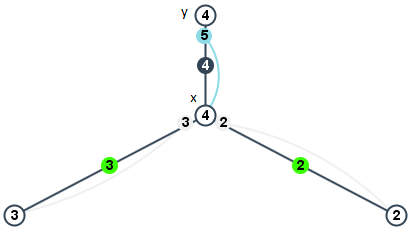
\includegraphics[width=0.65\textwidth]{bilder/abb_neu_max1max2.png}}
%	\hfill  
%lösche die neue line und füge das \hfill wieder ein um die bilder nebeneiander zu haben
	
	\subfigure[Da das Knotengewicht durch die Kante zwischen x und y bestimmt wird (grün), und dieses größer ist als die Summe der beiden normalen Kanten $edge_{1}$ und $edge_{2}$ (gelb), bestimmt diese Kante den Wert der Nachricht $\lambda_{y} = 5$ (blau). \label{modifiziert_b}]{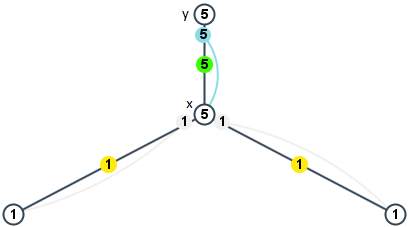
\includegraphics[width=0.65\textwidth]{bilder/abb_neu_edge.png}} 
%	\hfill
	
	\subfigure[Die größte Nachricht (grün), die an $x$ ankommt, ist größer als die bisher berechnete Nachricht und bestimmt daher den Nachrichtenwert $\lambda_{y} = 8$ (blau). \label{modifiziert_c}]{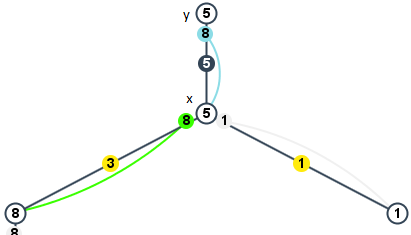
\includegraphics[width=0.65\textwidth]{bilder/abb_neu_msgData.png}}  
	
	\caption{Drei Fälle, die bei der Modifizierung des Algorithmus beachtet werden müssen, um alle Spezialfälle abzudecken. (Quelle: Eigene Darstellung im Applet)} 

\end{figure}

\subsubsection{Laufzeit}
	
	\begin{theorem}\label{thm_laufzeit_modifikation}
		Die Modifikationen des Algorithmus ändern nichts an der linearen Laufzeit.
	\end{theorem}
	\begin{proof}
		Die Grundidee des Algorithmus bleibt erhalten. Jeder Knoten schickt zu all seinen Nachbarn je eine Nachricht. Die Anzahl der Nachrichten ändert sich durch die Modifikation nicht, sondern nur ihre Berechnung.\\Die Berechnung kann in konstanter Zeit durchgeführt werden, dass pro Knoten nur drei Schritte notwendig sind:
		\begin{enumerate}
			\item Berechnung der Nachricht durch einfache Addition
			\item Vergleich der Nachricht (und evtl. Anpassen) mit dem Knotengewicht
			\item Vergleich der Nachricht (und evtl. Anpassen) mit der maximalen Nachricht
		\end{enumerate}
		Die lineare Zeit des als Grundlage verwendeten Algorithmus wurde im erwähnten Paper \cite{cima_paper} bereits bewiesen und kann in Theorem \ref{thm_laufzeit} nachgelesen werden.
	\end{proof}



